%-----------------------------------------------------------------------------------------------
\documentclass[addpoints, 11pt]{exam}
\usepackage[margin=.75in]{geometry}
\usepackage{etex}
\usepackage{graphicx}
\usepackage{amssymb}
\usepackage[final]{pdfpages}
\usepackage[fleqn]{amsmath}
\usepackage{nccmath}
\usepackage{cases}
\usepackage{hyperref}
\usepackage{multicol}
\usepackage{enumerate}
\usepackage{tikz}
\usepackage{pgfplots}
\usetikzlibrary{patterns}
\usepackage{pstricks-add}
%\usepackage{pst-func}
%\usepackage{pst-plot}
%\usepackage{pst-spectra}
\usepackage{multido}
\usepackage{lastpage}
\usepackage{ulem}
\usepackage[outside]{coordsys}
\usetikzlibrary{pgfplots.statistics}
\usetikzlibrary{positioning, shapes.geometric}
\usepackage{float}
%-------------------------------------------------------------------------------------------------
\setlength{\columnsep}{.5cm}
\setlength{\columnseprule}{1pt}
\newcommand{\ds}{\displaystyle}
\newcommand{\work}{{\bf{No Work $\Leftrightarrow$ No Points }}}
\newcommand{\neat}{{\bf{Use Pencil Only $\Leftrightarrow$ Be Neat \& Organized }}}
\newcommand{\answer}{\large\bf Ans: \underline{\hspace{1.5in}}}
\newcommand{\la}{\lambda}
\newcommand{\zz}{\mathbb{Z}}
\newcommand{\rr}{\mathbb{R}}
\newcommand{\nn}{\mathbb{N}}
\newcommand{\qq}{\mathbb{Q}}
\newcommand{\cc}{\mathbb{C}}
\newcommand{\cyclic}[1]{\langle #1 \rangle}
\newcommand{\lcm}{{\rm{lcm}}}
\renewcommand{\solutiontitle}{\noindent\textbf{Answer:}\par\noindent}
%------------------------------------------------------------------------------------------------
\begin{document}
%------------------------------------------------------------------------------------------------
\cfoot{UCLA: C. Johnson}
%	\rfoot{Total Points: \numpoints}
\rfoot{Page \thepage\ of \pageref{LastPage}}
%------------------------------------------------------------------------------------------------
\begin{center}
\fbox{%
	\parbox{1\linewidth}{%
		\noindent \Large\bfseries \\[.05in] Math 142: Modeling{\hspace{1.2in}{\Large\bfseries Name:{\hrulefill}}\\[.2cm]
			\noindent \Large\bfseries Homework \# 5 \hspace{2.8in}{Due:} Friday Nov 3
		}\\[.025in]
	}%
}
\end{center}
\addpoints


\vspace{.25cm}


%------------------------------------------------------------------------------------------------
\noindent  {\bf Directions} Complete the exercises. Your solutions to the exercises should be submitted to Gradescope before the indicated due date above. Please follow rules regarding Gradescope submission as described in the syllabus. \\


\noindent{\bf References} Except for the help of the instructor or TAs and the class textbooks and notes, if you use any resources, for example, a book, a website, or you discussed with your friends, please acknowledge them in this References section. 
\begin{itemize}
\item I discussed Problem ?? with STUDENT A, STUDENT B, $\ldots$
\item I used BOOK/WEBSITE to help me do Problem ??.
\end{itemize}
\vspace{.05cm}
%\hrule
%----------------------------------------------------------------------------------------------  
\noindent {\bf Exercises}
%\begin{multicols*}{2}
\begin{questions}
%----------------------------------------------------------------------------------------------  
%----------------------------------------------------------------------------------------------  
\question  {\bf Population genetics} We have argued that real populations have carrying capacities, at which rates of birth and death are equal. We can study the diversity of such populations (how many different cells will be present), using a Moran process model. Consider a population of $N$ cells, which we initially label $1,2,3, \ldots$. You task is to develop a simulation of how many descendants each of these starting cells has during the following process.\\

In each unit of time, imagine that a randomly chosen cell among the $N$ divides. This produces another cell with the same label (so if a cell with label 2 divides, then the new cell also has label 2). But to keep the number of cells constant, a cell must die. Take another randomly chosen cell among the $N$ and remove it from the population. (It is possible that the same cell will divide and die in a single time step - that's ok).
e.g. Suppose we start with 6 cells: $1,2,3, \ldots 6$ In our first step we find that cell 5 divides, and cell 2 dies. After the first step our cells are now labeled: $1,3,4,5,5,6$.
\begin{parts}
	\part Simulate 1000 time steps of this process using 6 cells. Show that after enough time steps all of the cells eventually have the same label (i.e. descend from only one of your starting cells).
	\part Simulate 100 replicate populations, each with $N=6$ cells. Show that they all, eventually each replicate population becomes homogeneous.
	\begin{figure}[H]
		\centering
		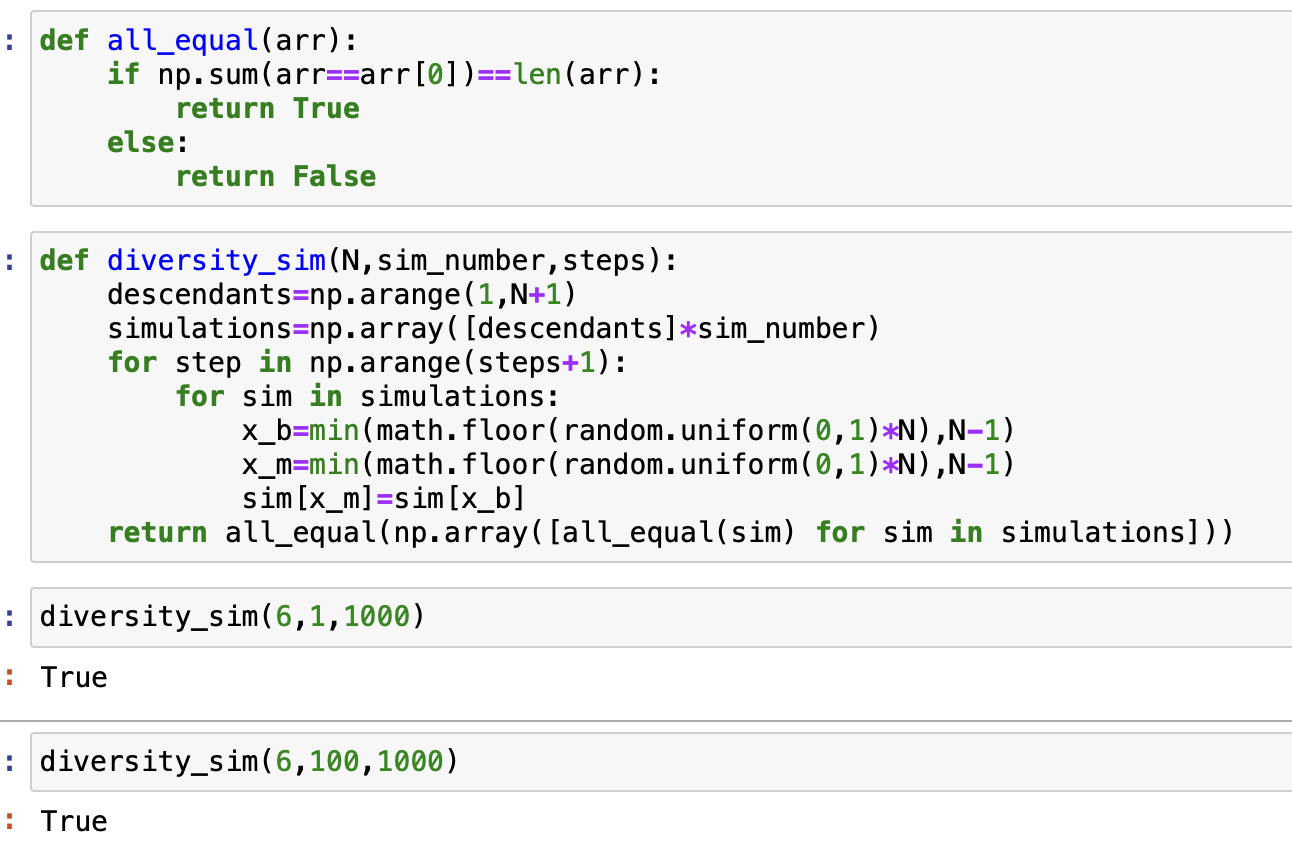
\includegraphics[scale=0.5]{Screenshot 2023-10-30 at 7.32.25 PM.png}
	\end{figure}
	(This answers both (a) and (b))
	\part Explain: After 1000 time steps, what is the average number of descendants that cell number 1 should have among the 6 cells? Argue mathematically (hint: every cell should have the same average number of descendants), and then compare with the answer obtained from your numerical simulation.\\
	If, on average, every cell should have the same number of descendants, we should expect each cell to produce $\frac{1000}{6}$ descendants. Using numerical simulations, we obtain an average of $199.43$ with distribution:
	\begin{figure}[H]
		\centering
		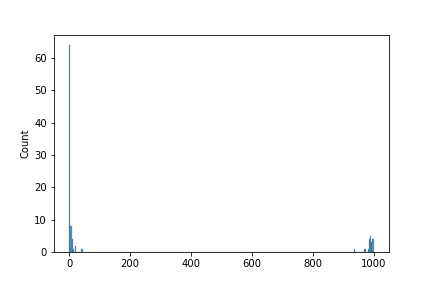
\includegraphics[scale=0.5]{div_sim_descendant_count.png}
	\end{figure}
	\part The same homogenization occurs in populations of different sizes. Measure the average time taken for the population to become homogeneous in $N=3, N=10, N=15$ cells.
	\begin{figure}[H]
		\centering
		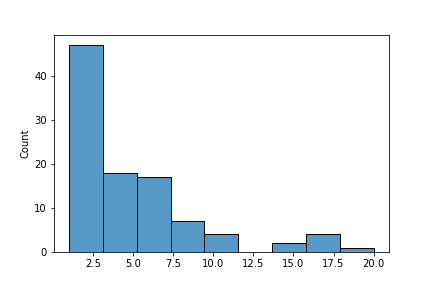
\includegraphics[scale=0.5]{div_sim_hom_3.png}
	\end{figure}
	N=3 mean=$5.02$
	\begin{figure}[H]
		\centering
		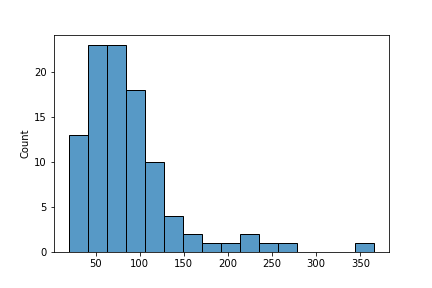
\includegraphics[scale=0.5]{div_sim_hom_10.png}
	\end{figure}
	N=10 mean $88.1$
	\begin{figure}[H]
		\centering
		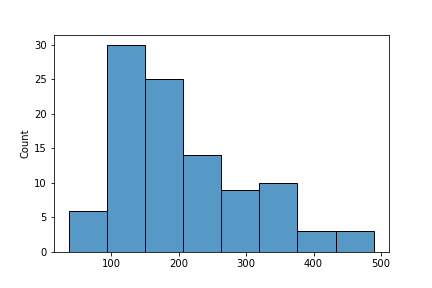
\includegraphics[scale=0.5]{div_sim_hom_15.png}
	\end{figure}
	N=15 mean $205.58$
	\part It has been argued that the average number of steps for the population to homogenize is proportional to $N^2$. Plot your data from (d) in a way that tests this relationship.
	The process of homogenization is known as genetic drift, and is an important force in evolution. Although our model is for cells dividing, it also occurs in populations that reproduce sexually. In particular we inherit our mitochondrial DNA is inherited directly from our mothers. Through mitochrondial DNA it can be shown that we are each descendants of one of between 7 and 29 women (different genetic mapping methods produce different answers).
	\begin{figure}[H]
		\centering
		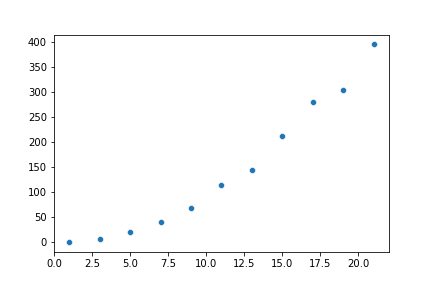
\includegraphics[scale=0.5]{div_sim_hom_rates.png}
	\end{figure}
	\begin{figure}[H]
		\centering
		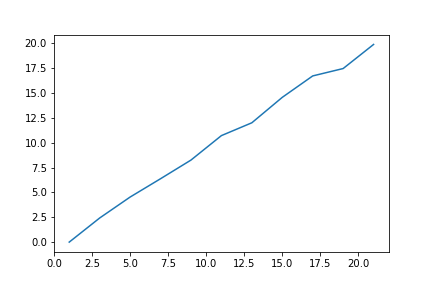
\includegraphics[scale=0.5]{div_sim_hom_regression.png}
	\end{figure}
	The scatter plot shows that there appears to be some evidence for a quadratic relationship. The relationship between the square roots of the average time it takes to reach homogenization vs. number of cells appears to be somewhat linear.
\end{parts}
%----------------------------------------------------------------------------------------------   
%----------------------------------------------------------------------------------------------  
\question  In class we studied the logistic model for the density dependent growth of populations:
$$
\frac{d N}{d t}=r\left(1-\frac{N}{K}\right) N, \quad N(0)=N_0,
$$
and we derived the solution:
$$
N(t)=\frac{K}{1-\frac{N_0-K}{N_0} e^{-r t}},
$$
and showed explicitly that $N(t) \rightarrow K$ as as $t \rightarrow \infty$, so long as $N_0>0$.
\begin{parts}
	\part Check explicitly that $N(0)=N_0$.\\
	$N(0)=\frac{K}{1-\frac{N_0-K}{N_0} e^{-r \cdot 0}}=\frac{K}{\frac{N_0}{N_0}-\frac{N_0-K}{N_0} \cdot 1}=\frac{K}{\frac{K}{N_0}}=N_0$
	\part Suppose that $N_0<K$. Show by computing $N^{\prime}(t)$, that $N(t)$ is an increasing function.\\
	$N'(t)=(K\cdot {(1-\frac{N_0-K}{N_0} e^{-r t})}^{-1})'=K(-1)\cdot {(1-\frac{N_0-K}{N_0} e^{-r t})}^{-2}\cdot r\frac{N_0-K}{N_0}e^{-rt}$\\
	$\frac{N_0-K}{N_0}<0$ because $N_0<K$, so let $P=-\frac{N_0-K}{N_0}$ be a positive number.\\
	Thus, $N'(t)=\frac{KPe^{-rt}}{{(1+Pe^{-rt})}^2}>0$ because $K,P,e^{-rt}>0$ for all $t$ and dividing a positive number by a positive number yields a positive number.
	Since $N'(t)\ge0$ for all $t$, $N(t)$ is an increasing function.
	\part Suppose that $N_0>K$. By computing $N^{\prime}(t)$, determine whether $N(t)$ is an increasing or decreasing function.
	$0<\frac{N_0-K}{N_0}<1$ because $N_0>K$, so let $P=\frac{N_0-K}{N_0}$ be a positive number.\\
	$N'(t)=\frac{-KP}{{(1-P e^{-r t})}^{2}}<0$ because $0<1-P e^{-r t}$ ($0<P,e^{-rt}<1\Rightarrow 0<P\cdot e^{-rt}<1$) and $-KP<0$.\\
	Since $N'(t)\le0$ for all $t$, $N(t)$ is an decreasing function.
	\part Suppose that $N_0=K$. What is the behavior of the solution?\\
	$\frac{N_0-K}{N_0}=0$ because $N_0=K$, so $N'(t)=0$. Thus, $N(t)=K$ is a constant function
\end{parts}
%----------------------------------------------------------------------------------------------   
\question Draw phase portraits and possible solution curves for the following autonomous differential equations:
\begin{parts}
	\part
	$$
	\frac{d x}{d t}=x^3-4 x .
	$$
	\part 
	$$
	\frac{d y}{d x}=y e^{-y}
	$$
	\part 
	$$\frac{d y}{d t}=\frac{y-2}{y^2-1} \quad, \quad y \neq \pm 1$$
	\part 
	$$
	\frac{d x}{d t}=\sin 2 x \quad, \quad 0 \leq x \leq 2 \pi
	$$
\end{parts}
%----------------------------------------------------------------------------------------------   
\question   Consider the ODE $\ds \frac{dy}{dt}=g(y)$. The graphs below are the graphs of $g(y)$. For each graph , draw the possible solution curves $y(t)$ as a function of $t$. Your sketch of the solution should show where the solution converges to (if it converges), and also where the solution curve is concave up, and also where it is concave down.

%---------------------------------------------------------------------------------------------- 
\question Look at the sets of solution curves shown in the graphs below. For each part, draw as well as you can, the corresponding phase portrait for the differential equation (that is, plot $g(y)$, the function on the right hand side of the differential equation $\left(\frac{d y}{d t}=g(y)\right)$.
------------------------------------------------------------------------------------
\question By separately graphing the two terms on the right hand side of each of the differential equations below, determine how many fixed points each equation has, and find their stability. (It is not necessary to find the numerical locations of any fixed points):
\begin{parts}
	\part
	$$
	\frac{d x}{d t}=e^{-x^2}-x,
	$$
	\part
	$$
	\frac{d y}{d t}=y^4-(1+y),
	$$
	\part
	$$
	\frac{d y}{d x}=y^3-e^{-y} .
	$$
	\begin{figure}[H]
		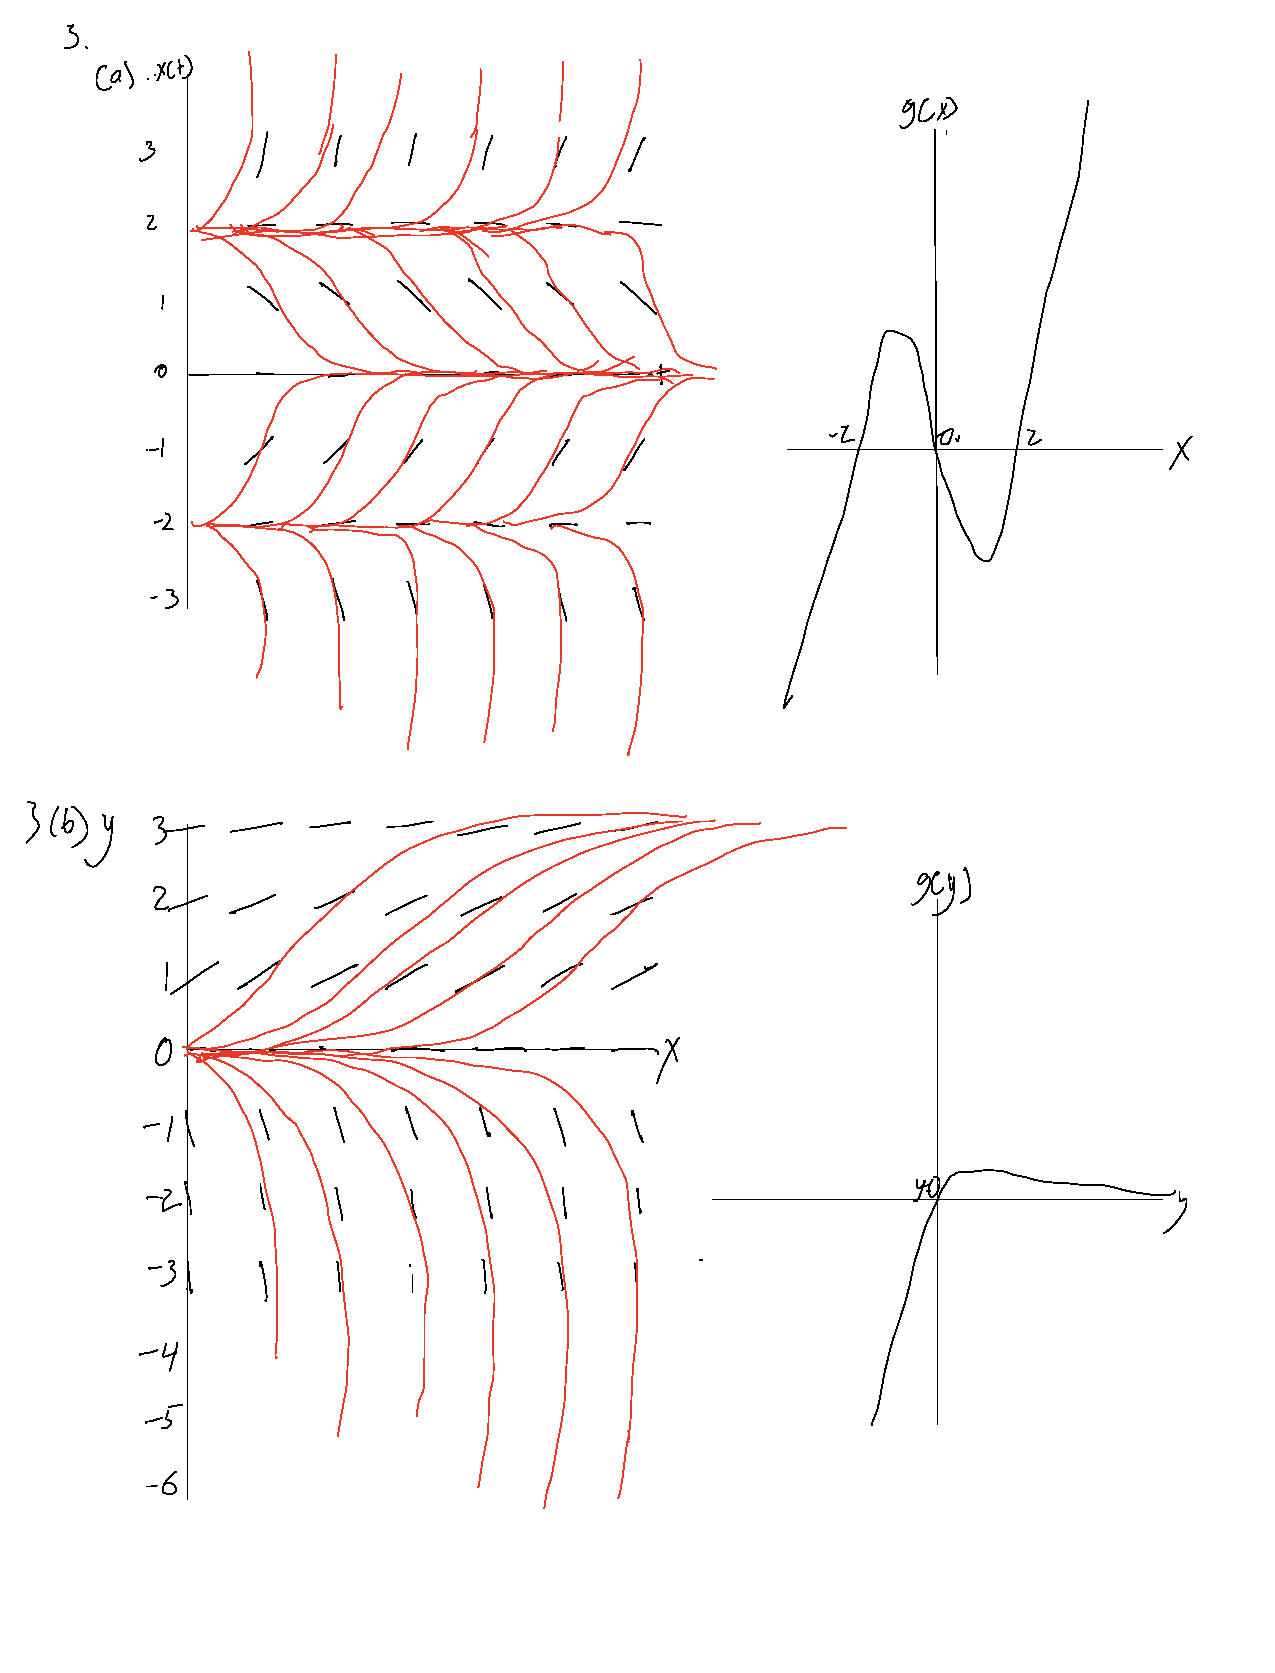
\includegraphics[page=1,scale=0.4]{Note Oct 29, 2023.pdf}
		\includegraphics[page=2,scale=0.4]{Note Oct 29, 2023.pdf}
		\includegraphics[page=3,scale=0.4]{Note Oct 29, 2023.pdf}
	\end{figure}
	\begin{figure}[H]
		\includegraphics[page=4,scale=0.4]{Note Oct 29, 2023.pdf}
		\includegraphics[page=5,scale=0.4]{Note Oct 29, 2023.pdf}
	\end{figure}
\end{parts}
%----------------------------------------------------------------------------------------------
\question Submit the code you used for any and all of the problems. (Print pdf the code) Either lump it all together at the end or when matching problems on Gradescope, select all pages of pdf that has code if you included code within the solution to each answer.
\begin{figure}[H]
	\centering
	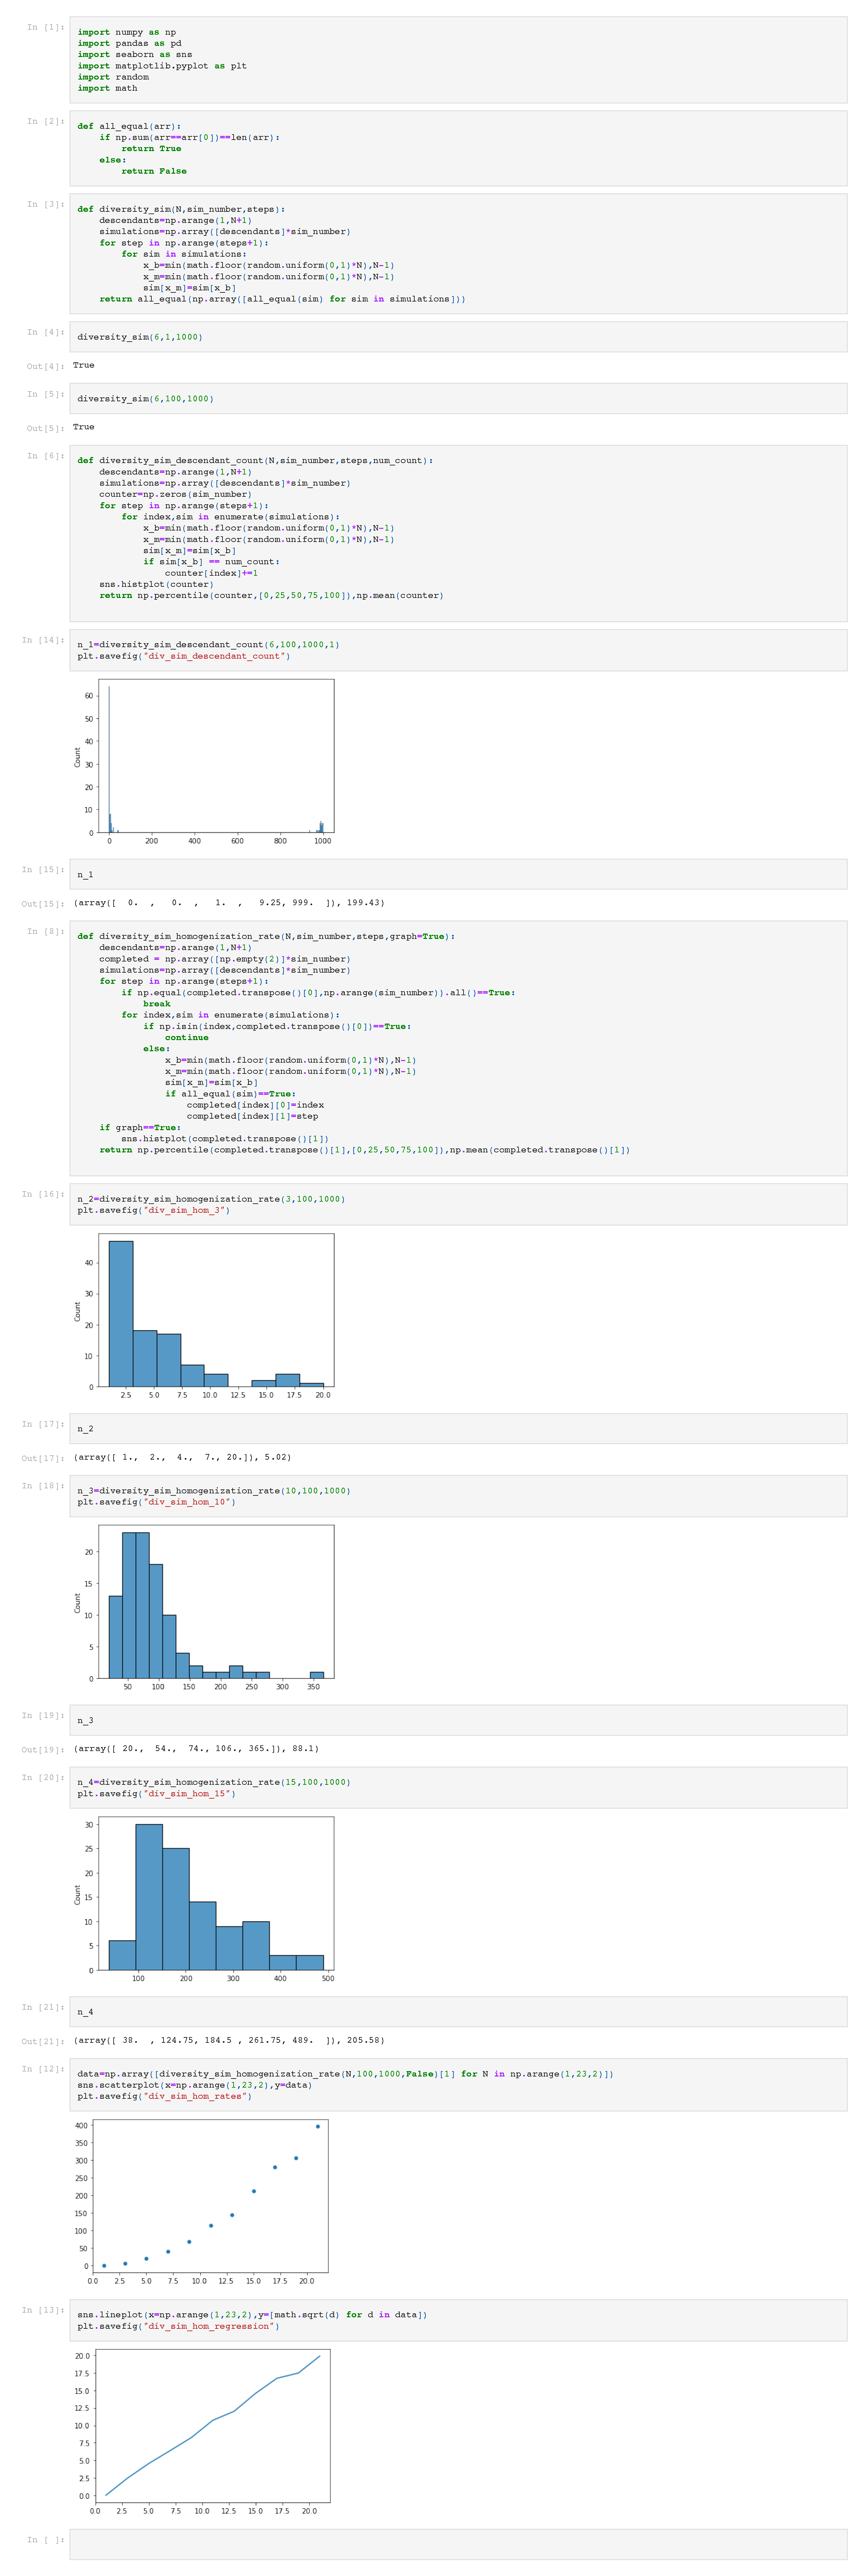
\includegraphics[scale=0.18]{Math 142 Homework 5 Q_1.pdf}
\end{figure}

%----------------------------------------------------------------------------------------------

\end{questions}
%\end{multicols*}
\end{document}